\newpage
\chapter*{Buzz Wire Game Instructions}
\addcontentsline{toc}{chapter}{Buzz Wire Game Instructions}

%
\section*{Step 1 Wiring (Positive and Negative)}
\addcontentsline{toc}{section}{Step 1 Wiring}

It is good practice to use two different coloured wires when you are wiring your ground and power rails in particular. The reason for this is that some components are polarised in that they have positive and negative sides. If you connect them the wrong way they will not work and could become damaged. To help avoid confusion later fill in the colours for each wire in the following section:

For my positive (+) connections I am using \makebox[3cm]{\hrulefill} colour wire.


For my negative (-) connections I am using \makebox[3cm]{\hrulefill} colour wire.


%
\begin{figure}[ht]
	\centering
	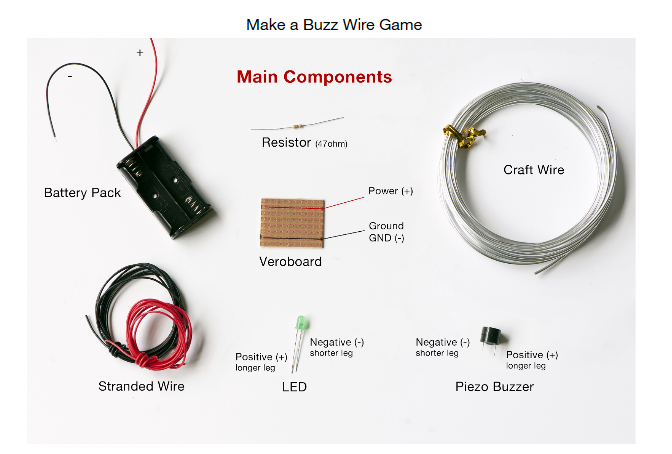
\includegraphics[width=8cm]{images/component_list}
	\caption{Buzz Wire Components List}
	\label{fig:components_list}
\end{figure}
%

\section*{Step 2 Prepare some wires}
\addcontentsline{toc}{section}{Step 2 Prepare some wires}

\begin{enumerate}
	\item Cut two lengths of positive wire about 15cm and strip both ends with wire strippers.
	
	\item Cute 2 lengths of negative wire about 15cm and strip both ends with wire strippers.
\end{enumerate}

%
\begin{figure}[ht]
	\centering
	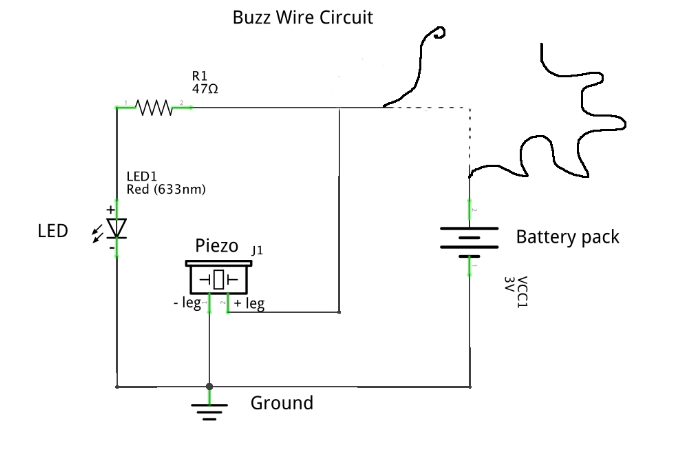
\includegraphics[width=8cm]{images/circuit_diagram}
	\caption{Buzz Wire Circuit Diagram}
	\label{fig:circuit_diagram}
\end{figure}
%


%
\section*{Step 3 The Piezo Buzzer}
\addcontentsline{toc}{section}{Step 3 The Piezo Buzzer}

Some components we are using have polarity. This means that they can only be connected to a circuit in one direction. Both the Piezo buzzer and the LED have positive and negative legs. The positive leg of the piezo buzzer is slightly longer than the negative leg, and additionally the positive side of the buzzer is also marked with a + symbol for easy identification.

\begin{enumerate}
	\item Solder one end of a stripped positive wire to the positive leg of the piezo buzzer. Then solder one of the stripped negative wires to the negative leg of the piezo.
	
	\item Thread both soldered wires through the wooden baseboard. Then flip the baseboard open.
	
	\item Solder the positive wire from the piezo to the power rail on your veroboard. To help you along we have marked one rail on the veroboard with tiny red dots on either end to mark the positive rail. You can use entire rail on the veroboard as all the holes in each row are connected.
	
	\item Similarly we have marked the negative rail with black dots. We recommend using this rail as your ground or negative rail. Solder the negative wire from the piezo to the ground rail on your veroboard.
\end{enumerate}

Congratulations your first component is in!!

%
\begin{figure}[ht]
	\centering
	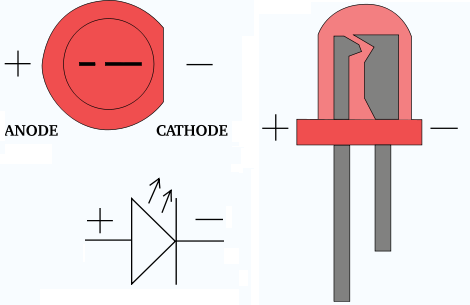
\includegraphics[width=8cm]{images/led}
	\caption{Buzz Wire Circuit Diagram}
	\label{fig:led}
\end{figure}
%


%
\section*{Step 4 The LED}
\addcontentsline{toc}{section}{Step 4 The LED}

The longer leg of the LED is the positive leg. It is called the anode (+). And the shorter leg is the negative leg. It is called the cathode (-). Examine the Figure:~\ref{fig:led} for more information about which is which.

\begin{enumerate}
	\item Thread the LED through the small hole nearest the piezo buzzer on the wooden base board.
	
	\item Solder one end of a stripped positive wire to the positive leg of the LED and solder one end of a stripped negative wire to the negative leg of the LED.
	
	\item Set aside for the moment.
\end{enumerate}


%
\section*{Step 5 The LED \& Resistor}
\addcontentsline{toc}{section}{Step 5 The LED \& Resistor}

The resistor component is non polarised which means that it does not have any positive or negative legs.

\begin{enumerate}
	\item Place the resistor in the veroboard with one leg in the power rail and another leg to some central rail in the centre of the veroboard.
	
	\item Solder the positive wire from the LED to any point along the same middle rail you just soldered the resistor to.
	
	\item Solder the negative wire from the LED to the ground rail on the veroboard.
\end{enumerate}

Congratulations you have two more components complete!



%
\section*{Step 6 The Battery Pack}
\addcontentsline{toc}{section}{Step 6 The Battery Pack}

The 3V AA battery pack comes pre-wired. The black wire is ground (-) and the red wire is the positive (+).

\begin{enumerate}
	\item Solder the black wire from the battery pack to the ground rail on the veroboard.
	\item Velcro your battery pack to the underside of your wooden base.
\end{enumerate}

%
\begin{figure}[ht]
	\centering
	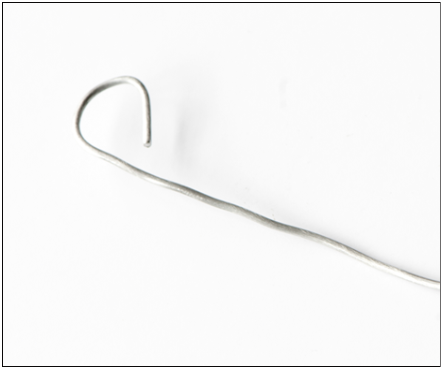
\includegraphics[width=8cm]{images/wand}
	\caption{Buzz wire wand}
	\label{fig:wand}
\end{figure}
%

%
\begin{figure}[ht]
	\centering
	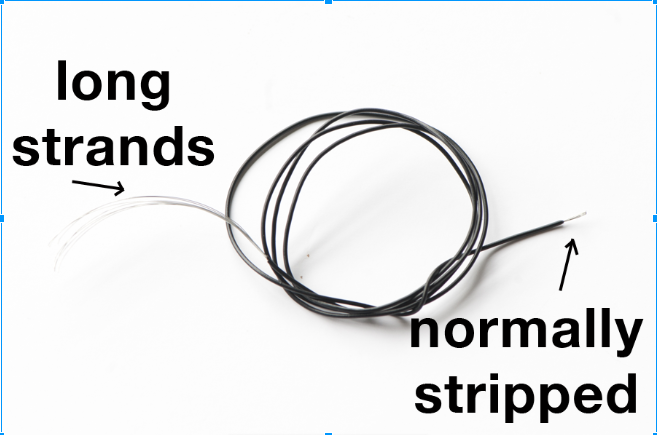
\includegraphics[width=8cm]{images/wand_cable}
	\caption{Buzz wire wand cable}
	\label{fig:wand_cable}
\end{figure}
%

%
\begin{figure}[ht]
	\centering
	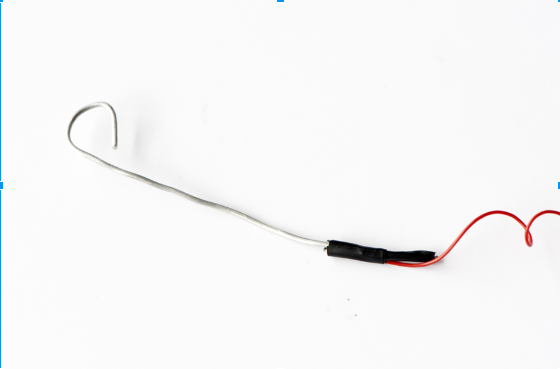
\includegraphics[width=8cm]{images/wand_cable_connected}
	\caption{Buzz wire wand and cable connected}
	\label{fig:wand_cable_connected}
\end{figure}
%

%
\section*{Step 7 Make the Wand}
\addcontentsline{toc}{section}{Step 7 Make the Wand}

\begin{enumerate}
	\item To get a good sounding 'buzz' from your craft wire you will need to sand it. Use some sandpaper and lightly sand all around your craft wire. This helps remove the thin coating on the outside and provide a better connection.
	
	\item Cut one piece of craft wire (about pencil length) for your wand. Make a hook at the top of your wand, leaving a small gap to easily slide on and off over the buzz wire. Set aside for the moment.
	
	\item To make the coiled wire for the wand you will need to cut a length of wire about 80cm long. One end of this wire can be stripped as normal. The other end will need to have a long length of stranded wire exposed.
	
	\item Wrap the middle section of this wire around a pencil. Hold with tape and heat with a hair dryer. This will coil the wire nicely and help prevent it from tangling like a telephone cord.
	
	\item Remove the pencil and solder the shorter stripped end of this coiled wire to the positive led on the battery pack.
	
	\item Wrap the longer stripped end around the base of the wand and securely fix with a little solder and some electrical tape for good measure.
\end{enumerate}


%
\section*{Step 8 Making the Bendy Buzz Wire}
\addcontentsline{toc}{section}{Step 8 Making the Bendy Buzz Wire}

\begin{enumerate}
	\item Push each end of the longer piece of craft wire through the remaining two holes on either end of the wooden base board. Bend into place at the back of the board.
	
	\item Like before, wrap one end of a piece of positive wire to one end of the buzz wire and securely fix with solder and some electrical tape.
	
	\item Solder the other end of this wire to the positive rail on the veroboard.
	
	\item Now the buzz wire is in a position where you can bend it into an interesting shape.	
\end{enumerate}


%
\section*{Step 9 Insert the Batteries}
\addcontentsline{toc}{section}{Step 9 Insert the Batteries}

The circuit is now complete! You can now insert the two AA batteries into the battery holder. Be sure to pay attention to the polarity of the batteries and insert them in the correct way!

Test to see if your circuit is working, touch the wand off the buzz wire, the LED should light and the piezo buzzer should sound off!

Have fun!






